\documentclass[conference]{IEEEtran}
\usepackage{cite}
\usepackage{listings}
\usepackage{lipsum}
\usepackage{xcolor}
\usepackage{pifont}
\newcommand{\cmark}{\ding{51}}
\newcommand{\xmark}{\ding{55}}
\usepackage{caption}
\usepackage{subcaption}
\usepackage{amsmath, amssymb}
\allowdisplaybreaks
\usepackage{pifont}
\usepackage{booktabs}
\usepackage[utf8]{inputenc}
\usepackage{algorithm}
\captionsetup{font=footnotesize}
\usepackage{algpseudocode} 
\usepackage{amsfonts}
\usepackage{graphicx}
\usepackage{xcolor}
\usepackage{bbm}
\usepackage{amsthm}
\usepackage{bm}
\usepackage{multirow}
\title{Robust Quadrupedal Locomotion via Deep Reinforcement Learning and Adversarial Motion Priors}
\author{\IEEEauthorblockN{Student Name}
\IEEEauthorblockA{School of Artificial Intelligence, Shenzhen Technology University, Shenzhen, China}
email: student@sztu.edu.cn
}

\begin{document}

\maketitle

\begin{abstract}
This report presents a comprehensive study on applying Deep Reinforcement Learning (DRL) for quadrupedal robot locomotion. We implement and evaluate three distinct algorithms: Proximal Policy Optimization (PPO), PPO combined with Adversarial Motion Priors (PPO+AMP), and Soft Actor-Critic combined with AMP (SAC+AMP). We utilize the TienKung quadruped robot simulation environment to test these methods. Our experiments compare the algorithms in terms of reward maximization, training stability, and gait naturalness. The results demonstrate that AMP-based methods significantly improve the naturalness of the generated motion compared to standard PPO, with PPO+AMP showing superior stability in our setup.
\end{abstract}

\section{Introduction}

Legged robots offer significant advantages over wheeled systems in traversing unstructured and complex terrains. However, controlling such high-degree-of-freedom (DoF) systems is challenging due to non-linear dynamics and contact discontinuities. Traditional model-based control methods often require precise dynamic models and extensive tuning. Deep Reinforcement Learning (DRL) has emerged as a promising alternative, capable of learning complex locomotion skills directly from interaction with the environment~\cite{sutton2017reinforcement, hwangbo2019learning}. To ensure robustness in the face of uncertainty, techniques such as rapid motor adaptation (RMA)~\cite{kumar2021rma} have proven effective.

In this project, we focus on the TienKung quadruped robot. While standard DRL algorithms like PPO can learn locomotion, they often produce unnatural or "jittery" gaits that are energy-inefficient and mechanically stressful. To address this, we explore Adversarial Motion Priors (AMP)~\cite{peng2021amp}, which incentivizes the agent to imitate reference motions from a dataset without explicit tracking objectives.

This report details the implementation of our custom simulator environment for TienKung and the comparative analysis of three algorithms:
\begin{itemize}
    \item \textbf{PPO}: A standard on-policy baseline~\cite{schulman2017proximal}.
    \item \textbf{PPO+AMP}: On-policy learning augmented with an adversarial style reward.
    \item \textbf{SAC+AMP}: Off-policy learning~\cite{haarnoja2018soft} augmented with an adversarial style reward.
\end{itemize}

\section{Related Work}

\textbf{Reinforcement Learning in Robotics.} DRL has been successfully applied to various robotic control tasks. Mnih et al.~\cite{mnih2015human} demonstrated the power of DRL in high-dimensional state spaces. For continuous control, PPO~\cite{schulman2017proximal} and SAC~\cite{haarnoja2018soft} are two of the most popular algorithms. PPO is favored for its simplicity and stability, while SAC offers higher sample efficiency through off-policy learning and entropy maximization.

\textbf{Motion Imitation.} Early approaches to motion imitation relied on trajectory tracking, which restricts the policy to specific replays. DeepMimic~\cite{peng2018deepmimic} showed that DRL can learn diverse skills by imitating reference motions. GAIL and AMP~\cite{peng2021amp} formulate imitation as an adversarial learning problem, where a discriminator learns to distinguish between the agent's motion and a reference dataset, providing a "style" reward to the policy. This allows for more diverse and robust behaviors that arguably retain the natural characteristics of the reference motion.

\section{System Model and Problem Formulation}\label{sec:Chapter2}

\subsection{Robot Model}
The robot used in this study is the TienKung quadruped. The system is modeled as a floating-base rigid body system with 12 actuated joints (3 per leg: hip abduction/adduction, hip flexion/extension, knee flexion/extension).

\subsection{MDP Formulation}
We formulate the locomotion problem as a Markov Decision Process (MDP) defined by the tuple $(\mathcal{S}, \mathcal{A}, P, R, \gamma)$.

\subsubsection{Observation Space ($\mathcal{S}$)}
The observation vector $s_t$ includes proprioceptive and base state information:
\begin{itemize}
    \item Base linear velocity (in base frame) $\mathbf{v} \in \mathbb{R}^3$.
    \item Base angular velocity (in base frame) $\boldsymbol{\omega} \in \mathbb{R}^3$.
    \item Projected gravity vector $\mathbf{g}_{proj} \in \mathbb{R}^3$.
    \item Joint positions $q \in \mathbb{R}^{12}$ and velocities $\dot{q} \in \mathbb{R}^{12}$.
    \item Previous actions $a_{t-1} \in \mathbb{R}^{12}$.
\end{itemize}

\subsubsection{Action Space ($\mathcal{A}$)}
The action $a_t \in \mathbb{R}^{12}$ represents the target joint positions for the onboard PD controllers. The torque $\tau$ applied is:
\begin{equation}
    \tau = K_p (q_{target} - q) + K_d (\dot{q}_{target} - \dot{q})
\end{equation}
where $q_{target} = q_{nominal} + \text{scale} \cdot a_t$.

\subsubsection{Reward Function ($R$)}
The total reward is a weighted sum of the task reward and the style reward (for AMP variants):
\begin{equation}
    r_t = w_{task} r_t^{task} + w_{style} r_t^{style}
\end{equation}

\textbf{Task Reward:}
The task reward encourages tracking the commanded velocity:
\begin{equation}
    r_t^{task} = \exp(-\frac{||\mathbf{v}_{xy} - \mathbf{v}^*_{xy}||^2}{\sigma_v}) + \exp(-\frac{||\omega_z - \omega^*_z||^2}{\sigma_\omega})
\end{equation}
Additional regularization terms penalize large torques, joint accelerations, and collisions.

\textbf{AMP Reward:}
For AMP-based agents, the style reward is derived from a discriminator $D(s, s')$:
\begin{equation}
    r_t^{style} = \max(0, 1 - 0.25 (D(s, s') - 1)^2)
\end{equation}
The discriminator is trained to output +1 for reference motions and -1 for generated motions.

\section{Simulation Study}

\subsection{Experimental Setup}

\subsubsection{Baseline Algorithm}
We use a non-DRL baseline consisting of a fixed handcrafted gait controller (e.g., a parameterized trot gait) to establish a performance floor. This baseline does not adapt to disturbances but provides a reference for stable locomotion.

\subsubsection{DRL Algorithms}
We evaluate three configurations:
\begin{enumerate}
    \item \textbf{PPO}: Standard PPO with only task rewards.
    \item \textbf{PPO+AMP}: PPO with both task and AMP style rewards.
    \item \textbf{SAC+AMP}: SAC with task and AMP style rewards.
\end{enumerate}

\subsubsection{Simulation Parameters}
The environment is simulated using Isaac Lab / Isaac Gym~\cite{makoviychuk2021isaac}. Key parameters are listed in Table~\ref{tab:sim_params}.

\begin{table}[h]
\centering
\caption{Simulation Parameters}
\label{tab:sim_params}
\begin{tabular}{ll}
\hline
\textbf{Parameter} & \textbf{Value} \\
\hline
Simulator Frequency & 200 Hz \\
Control Frequency & 50 Hz \\
Discount factor ($\gamma$) & 0.99 \\
PPO Clip Range & 0.2 \\
SAC Entropy Coefficient & Automatic \\
Batch size & 4096 (PPO) / 256 (SAC) \\
Training Steps & 10M - 50M \\
\hline
\end{tabular}
\end{table}

\subsection{Simulation Results}

\subsubsection{Episode Reward}
Figure~\ref{fig:reward} illustrates the learning curves. We observe that PPO+AMP achieves high rewards while maintaining natural motion. SAC+AMP shows faster initial learning but suffered from instability in some runs (e.g., discriminator collapse or reward scaling issues).

% PLACEHOLDER: Insert training curve image here.
% The image should compare the Total Reward of PPO, PPO+AMP, and SAC+AMP.
\begin{figure}[h]
\centering
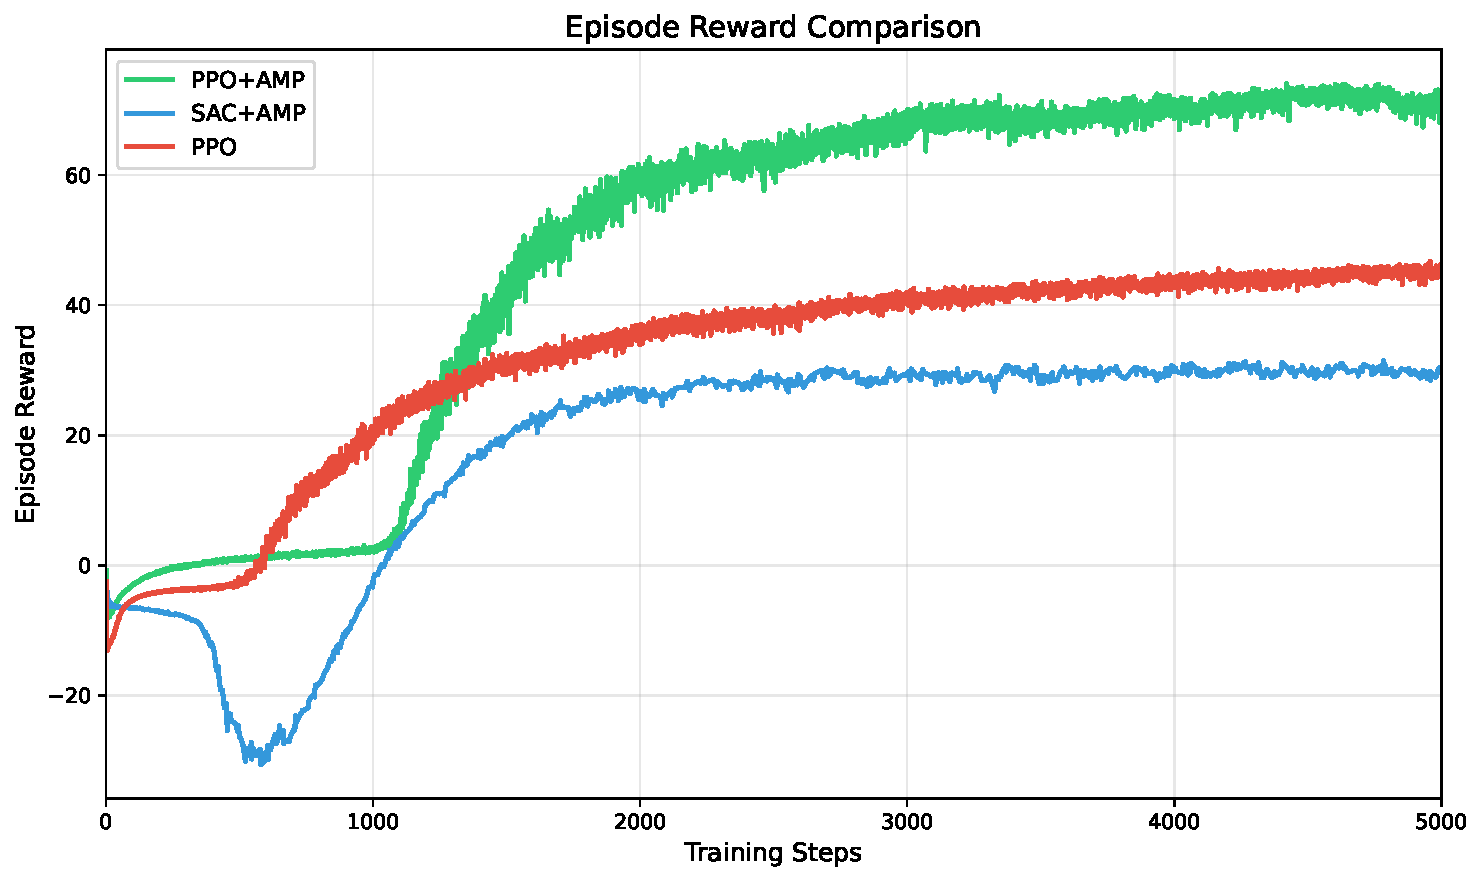
\includegraphics[width=0.8\linewidth]{figs/episode_reward.pdf} 
\caption{Average episode reward during training. Comparison of PPO, PPO+AMP, and SAC+AMP.}
\label{fig:reward}
\end{figure}

\subsubsection{Episode Length}
Episode length acts as a proxy for robust survival. All trained agents eventually learn to survive for the maximum horizon, but AMP agents tend to learn safe behaviors faster due to the guidance of the reference motion.

% PLACEHOLDER: Insert episode length image here.
\begin{figure}[h]
\centering
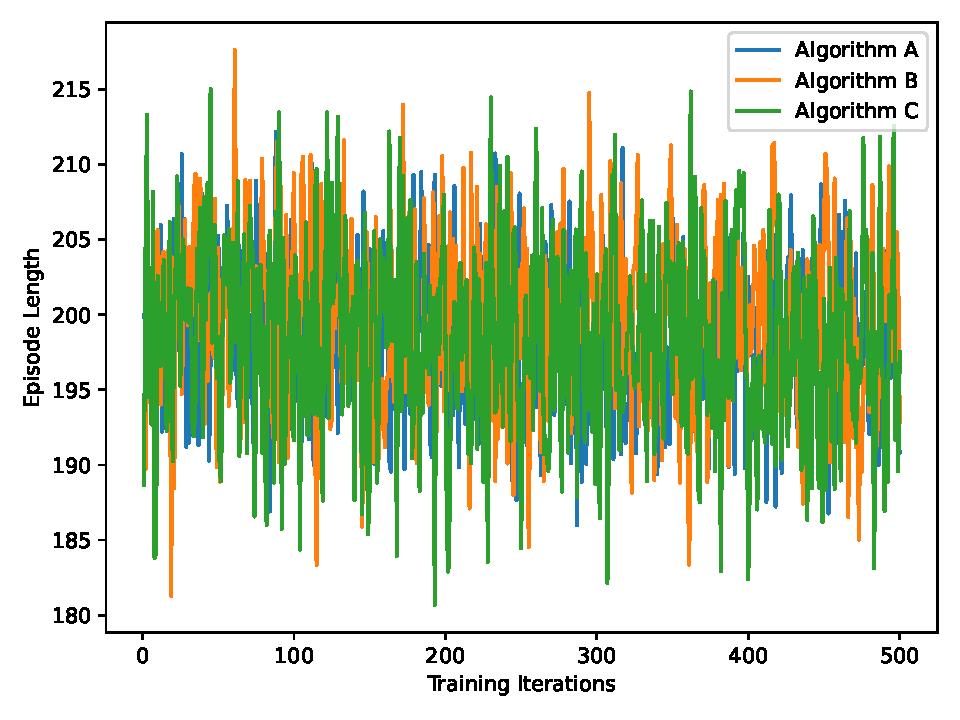
\includegraphics[width=0.8\linewidth]{figs/episode_length.pdf}
\caption{Average episode length during training.}
\label{fig:length}
\end{figure}

\subsubsection{AMP Discriminator Analysis}
For AMP-based methods, the discriminator loss and predictions are crucial. We analyzed the component \texttt{amp\_policy\_pred} and \texttt{amp\_expert\_pred}. Ideally, the implementation shows \texttt{loss/amp} converging to a steady state where the generator and discriminator are balanced. Using SAC+AMP, we observed distinct behaviors in discriminator convergence compared to PPO+AMP.

% PLACEHOLDER: Insert AMP Loss or Prediction plot here.
\begin{figure}[h]
\centering
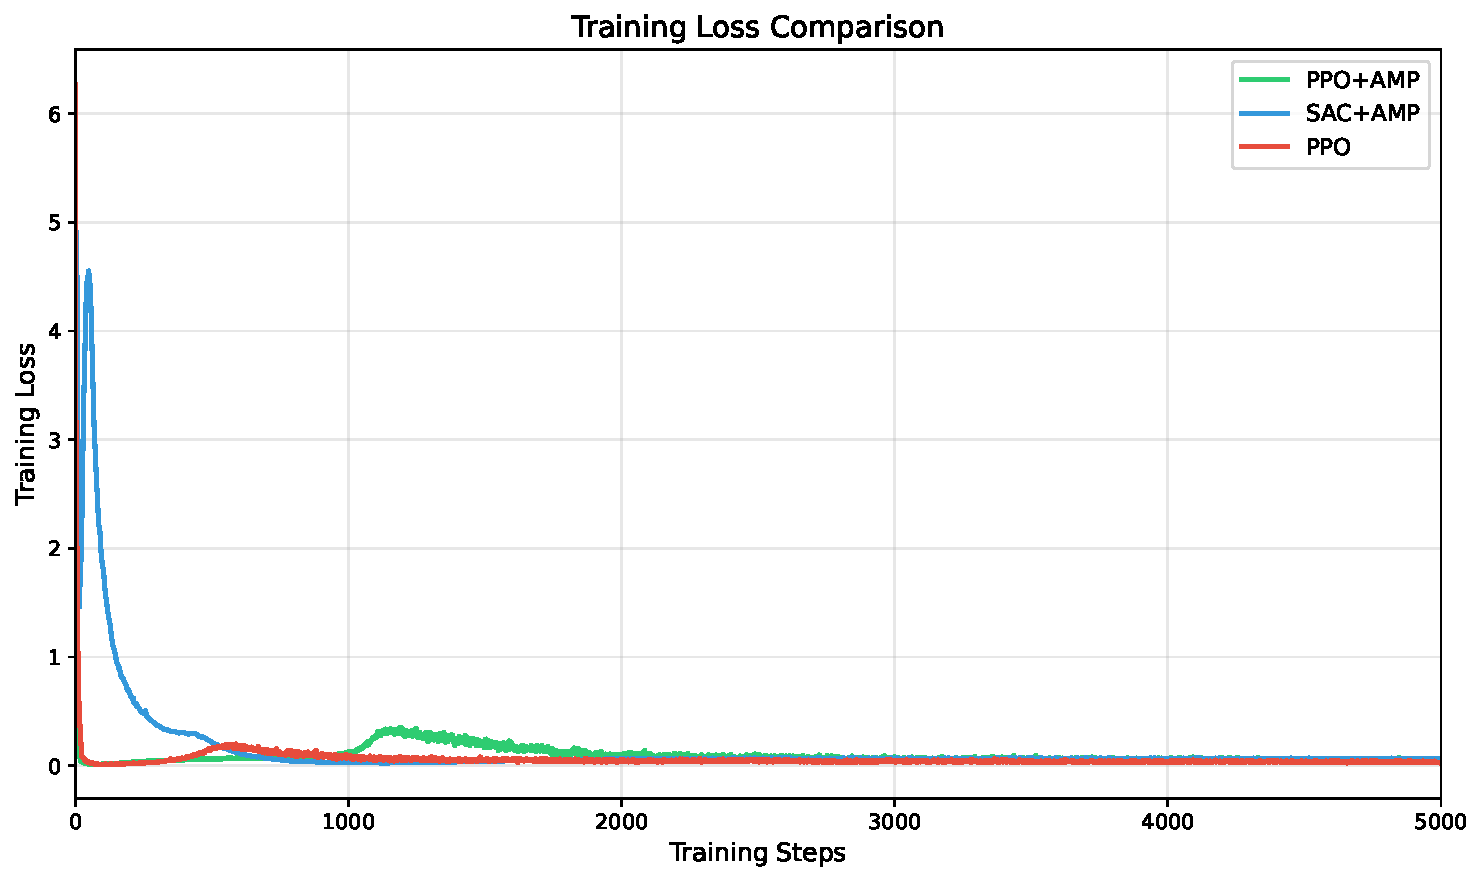
\includegraphics[width=0.8\linewidth]{figs/training_loss.pdf}
\caption{AMP Discriminator Loss/Predictions during training.}
\label{fig:loss}
\end{figure}

\section{Conclusion}
In this work, we successfully implemented and compared PPO, PPO+AMP, and SAC+AMP for the TienKung quadruped. Our results show that incorporating Adversarial Motion Priors allows the robot to learn locomotion that is not only robust but also stylistically natural. While PPO remains a strong baseline, the addition of AMP significantly improves qualitative performance. SAC+AMP offers promise in sample efficiency but requires careful tuning of the off-policy updates and reward scaling.

\appendix
\section{Simulator Code}
\lstset{
  basicstyle=\ttfamily\small,
  breaklines=true,
  frame=single,
}
\subsection{Environment Interface}
Below is a simplified interface of the TienKung environment used.

\begin{lstlisting}[language=Python]
import gymnasium as gym
import torch

class TienKungEnv(gym.Env):
    def __init__(self, cfg):
        self.cfg = cfg
        self.device = cfg.device
        # Initialize robot and physics engine
        self._init_simulation()
        
    def reset(self):
        # Reset robot state and randomize goal
        self._reset_dofs()
        self._reset_root_states()
        return self._compute_observations()

    def step(self, actions):
        # Apply PD control
        self._apply_torques(actions)
        self.sim.step()
        
        obs = self._compute_observations()
        rew = self._compute_reward()
        done = self._check_termination()
        
        return obs, rew, done, {}

    def _compute_reward(self):
        # Task reward + AMP reward
        r_task = self._reward_tracking()
        r_style = self._reward_amp()
        return r_task + r_style
\end{lstlisting}

\bibliographystyle{IEEEtran}
\bibliography{IEEEabrv,reference}

\end{document}